\section{Arbitrage Pricing Theory}
\label{sec:arbitrage_pricing_theory}
In this section we'll briefly discuss Arbitrage Pricing Theory (APT), and how it generalizes the Capital Asset Pricing Model (CAPM) as well as 
how Fama-Macbeth regressions can be used to estimate risk premia. The purpose of this section is not to be comprehensive,
but to briefly introduce concepts, as well as the code used when implementing portfolios in a systematic risk framework.

\subsection{Arbitrage Pricing Theory}
We've discussed \citet{fama_french_1993} and the Size and Value risk factors it proposes.
Throughout the article so far we've focused on one source of systematic risk, market risk.
From now on we will include the Size and Value factors in our equation for expected returns.

This multi-factor model has the form as per Equation~{\ref{eq:multi_factor}}. This is the model given by Arbitrage Pricing Theory (APT).

\begin{equation}
    \label{eq:multi_factor}
    E[R_i] = R_f + \beta_{i,m} \gamma_m + \beta_{i,s} \gamma_s + \beta_{i,v} \gamma_v
\end{equation}
Where:
\begin{itemize}
    \item $E[R_i]$ is the expected return of asset $i$
    \item $R_f$ is the risk-free rate
    \item $\beta_{i,m}$ is the asset's exposure to the market risk factor
    \item $\beta_{i,s}$ is the asset's exposure to the size risk factor
    \item $\beta_{i,v}$ is the asset's exposure to the value risk factor
    \item $\gamma_m$ is the market risk premium
    \item $\gamma_s$ is the size risk premium
    \item $\gamma_v$ is the value risk premium
\end{itemize}

For an asset $i$, the expected return is a function of its exposure to the market, size, and value risk factors, as represented by the Betas.
Risk premia are the expected returns of the systematic risk factors, and they are the same for all assets. Recall in the CAPM model, we were concerned only with
the market risk premium, now we have three risk premia.

Table ~\ref{tab:sample_asset_exposures} shows the exposures of a few sample assets to the market, size and value risk factors.

\begin{table}
    \centering
    \begin{tabular}{lccccc}
\toprule
Mkt-RF\_loading & SMB\_loading & HML\_loading & symbol \\
\midrule
1.113 & -0.251 & -0.379 & AAPL \\
0.983 & 0.140 & 0.582 & GE \\
0.804 & -0.147 & 0.335 & IBM \\
0.550 & -0.333 & 0.216 & KO \\
1.168 & -0.404 & -0.449 & MSFT \\
\bottomrule
\end{tabular}

    \caption{Sample assets and their exposures to the market, size and value risk factors}
    \label{tab:sample_asset_exposures}
\end{table}

We used to get the market risk premia by taking the average market return over our data period, but we will now introduce a way to get
the risk premia for the size and value factors.

\subsection{Fama-Macbeth Regressions}
Fama-Macbeth regressions are a two stage process that allows us to get the risk premia and factor sensitivities for a set of risk factors.

The first stage is a cross-sectional regression of the asset returns against the risk factors.
This gives us the factor sensitivities (betas) for each asset.
The second stage is a time-series regression of the factor sensitivities against the risk factors.
This gives us the risk premia for each factor at every time-step T.

Stage 1 is given by Equation~{\ref{eq:stage_1}}:
\begin{equation}
    \label{eq:stage_1}
    R_i = \alpha + \beta_{i,m} R_m + \beta_{i,s} R_s + \beta_{i,v} R_v + \epsilon
\end{equation}
Where:
\begin{itemize}
    \item $R_i$ is the return of asset $i$
    \item $\alpha$ is the intercept of the regression line
    \item $\beta_{i,m}$ is the asset's exposure to the market risk factor
    \item $\beta_{i,s}$ is the asset's exposure to the size risk factor
    \item $\beta_{i,v}$ is the asset's exposure to the value risk factor
    \item $R_m$ is the market return
    \item $R_s$ is the size return
    \item $R_v$ is the value return
    \item $\epsilon$ is the error term
\end{itemize}
The second stage is given by Equation~{\ref{eq:stage_2}}, where we're estimating the gammas using the betas from the first stage at every time period
t.
\begin{equation}
    \label{eq:stage_2}
    R_t = \gamma_{0,t} + \gamma_{m,t} \beta_{i,m} + \gamma_{s,t} \beta_{i,s} + \gamma_{v,t} \beta_{i,v} + \epsilon_t
\end{equation}
Where:
\begin{itemize}
    \item $R_t$ is the return of the portfolio at time $t$
    \item $\gamma_{0,t}$ is the intercept of the regression line at time $t$
    \item $\gamma_{m,t}$ is the market risk premium at time $t$
    \item $\gamma_{s,t}$ is the size risk premium at time $t$
    \item $\gamma_{v,t}$ is the value risk premium at time $t$
    \item $\epsilon_t$ is the error term at time $t$
\end{itemize}

We then take an average of the timeseries regression coefficients to get the risk premia for each factor.
These risk premia are also referred to as factor returns, since they are the expected returns of the risk factors.

If we take the cumulative sum of these risk premia coefficients, we can visually see the performance of the risk factors over time.
We can see this in figure \ref{fig:factor_returns}, where we plot the cumulative sum of the risk premia for the size and value factors.
\begin{figure}
    \centering
    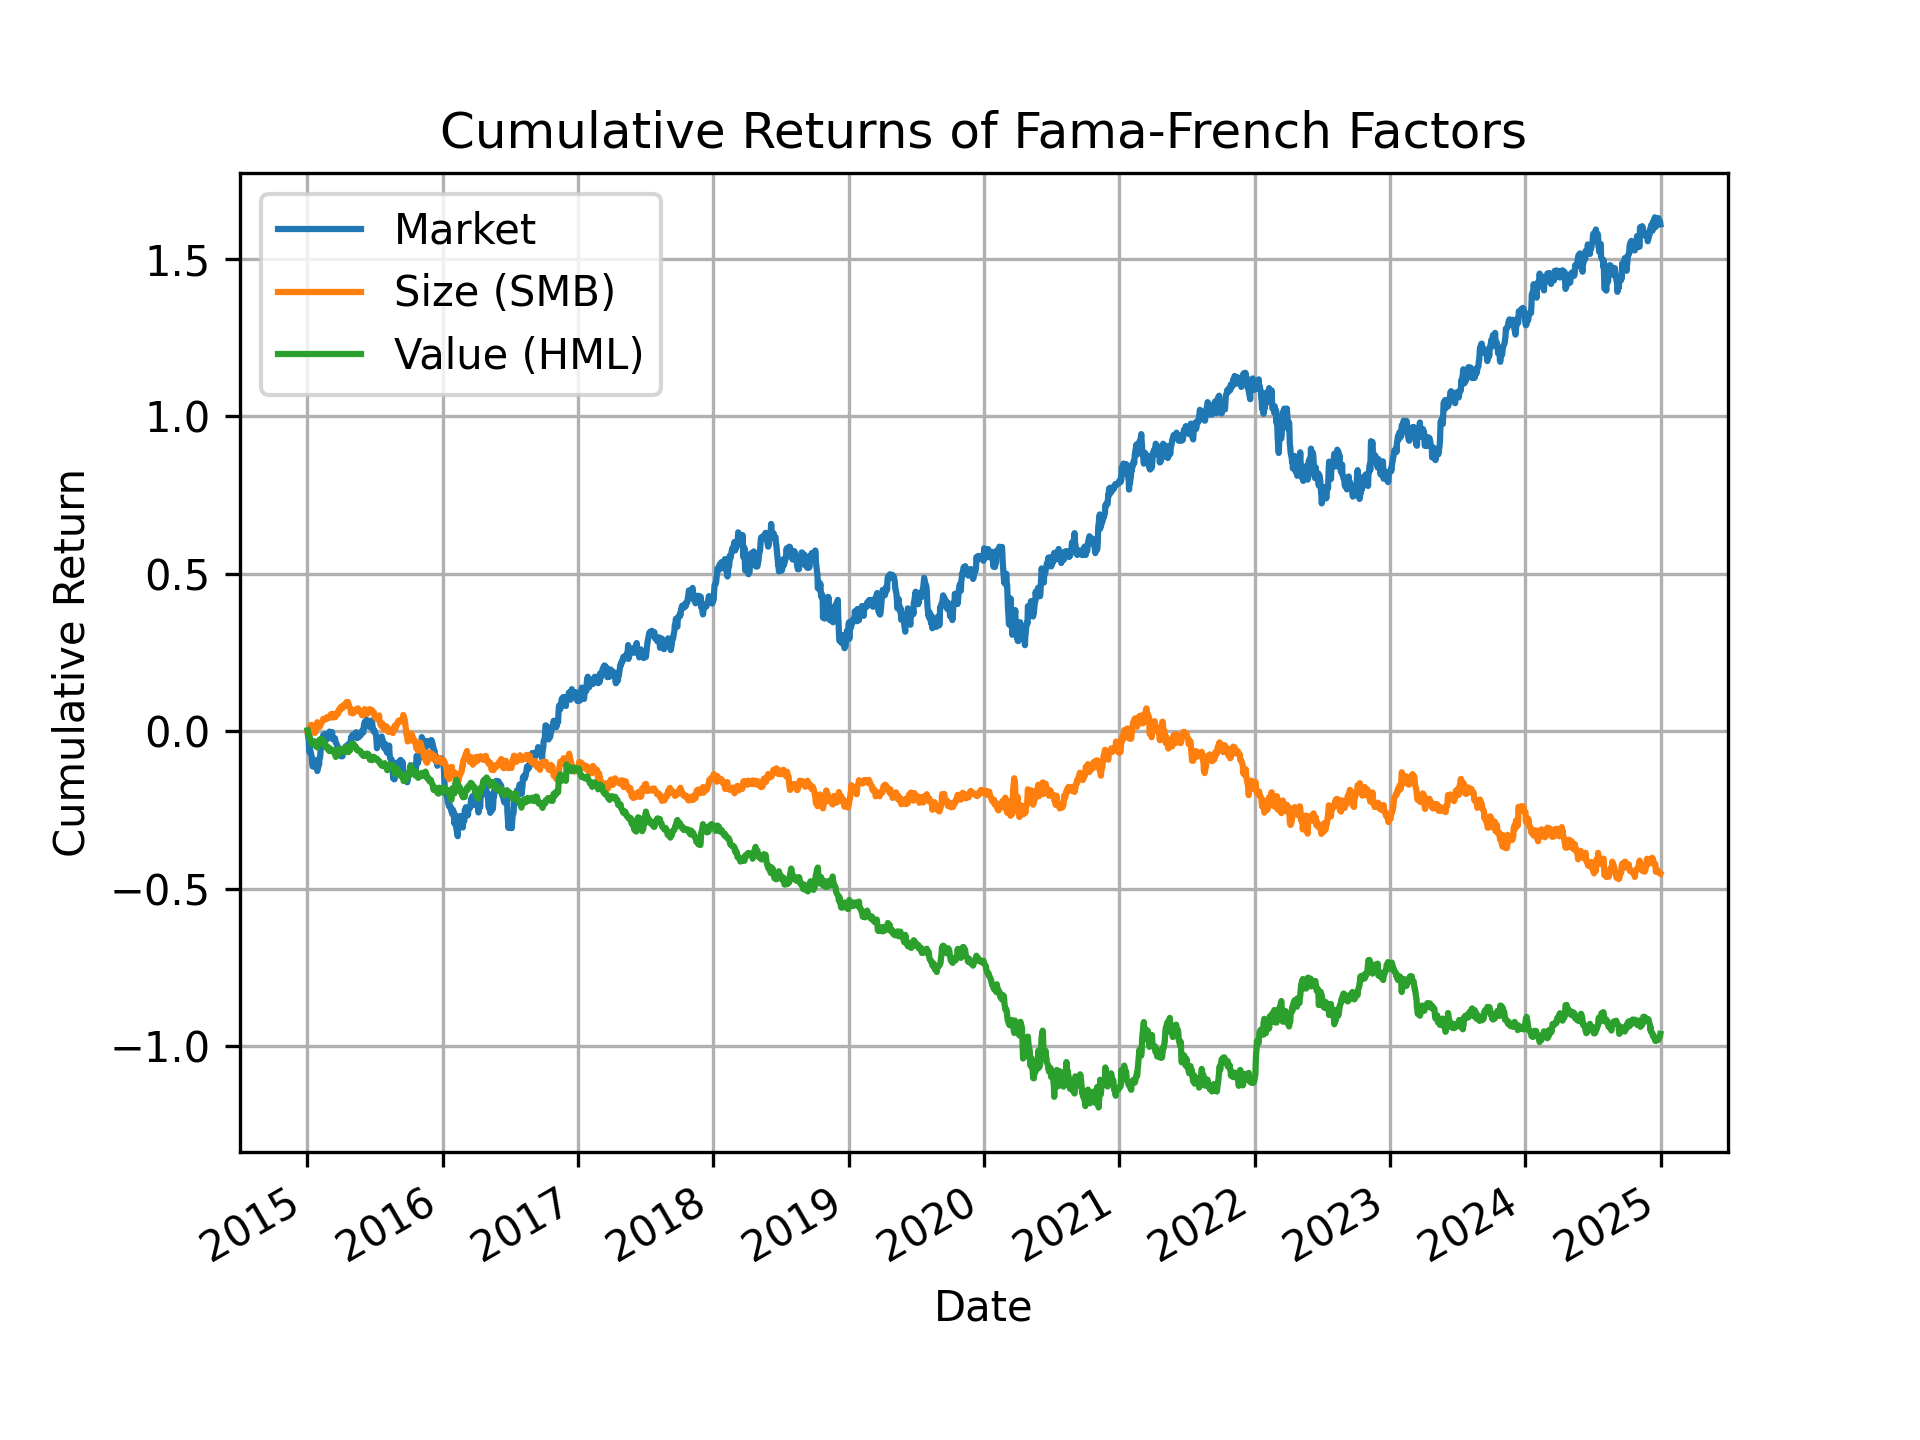
\includegraphics[width=0.8\textwidth]{../figs/factor_returns.png}
    \caption{Plot showing the cumulative sum of the risk premia for the market, size and value factors}
    \label{fig:factor_returns}
\end{figure}

We can take the averages of these coefficients to get the risk premia for each factor. The results are shown in table \ref{tab:expected_factor_returns}.
The negative premia we see on size and value factors come from a mix of using a small sample of assets, namely the bias from using the current constituents S\&P 500, our relatively short
lookback period of 10 years, and how value has underperformed in the ast few years.

We need two parts to construct portfolios, expected returns and risk.
We can get the expected returns from the Fama-Macbeth regressions, and we now, since we 
believe that returns are only a function of risk factors, we can use the covariance matrix of the risk factors to get the risk of the portfolio.
This greatly reduces the dimensionality of the problem, since we only need to estimate the covariance matrix of the risk factors, and not the covariance matrix of the assets.
Expected returns for APT portfolios are still weighted sums of the expected returns of the component assets. Risk is given slightly differently, as we are now using the covariance matrix of the risk factors, and not the covariance matrix of the assets.
The expected risk is given by Equation~{\ref{eq:apt_portfolio_risk}}:
\begin{equation}
    \label{eq:apt_portfolio_risk}
    \sigma_p^2 = w^T \Sigma w
\end{equation}
Where:
\begin{itemize}
    \item $\sigma_p^2$ is the variance of the portfolio
    \item $w$ is the vector of weights of the assets in the portfolio
    \item $\Sigma$ is the covariance matrix of the risk factors
\end{itemize}

Table~\ref{tab:apt_expected_returns} shows the expected returns for a few sample assets.
Table~\ref{tab:factor_cov_matrix} shows the covariance matrix of the risk factors.

\begin{table}
    \centering
    \vspace{1em}
    \begin{tabular}{lr}
\toprule
Factors & Expected Factor Returns \\
\midrule
Mkt-RF\_loading\_premium & 0.1612 \\
SMB\_loading\_premium & -0.0453 \\
HML\_loading\_premium & -0.0962 \\
\bottomrule
\end{tabular}

    \caption{Expected factor returns for the market, size and value factors}
    \label{tab:expected_factor_returns}
    \vspace{1em}
\end{table}
\begin{table}
    \centering
    \vspace{1em}
    \begin{tabular}{lr}
\toprule
symbol & expected\_return \\
\midrule
A & 0.17 \\
AAPL & 0.23 \\
ABBV & 0.10 \\
ABNB & 0.19 \\
ABT & 0.16 \\
\bottomrule
\end{tabular}

    \caption{Expected returns according to APT for a few sample assets}
    \label{tab:apt_expected_returns}
    \vspace{1em}
\end{table}
\begin{table}
    \centering
    \vspace{1em}
    \begin{tabular}{lrrr}
\toprule
 & Mkt-RF\_premium & SMB\_premium & HML\_premium \\
\midrule
Mkt-RF\_premium & 0.06 & 0.00 & -0.00 \\
SMB\_premium & 0.00 & 0.02 & 0.00 \\
HML\_premium & -0.00 & 0.00 & 0.02 \\
\bottomrule
\end{tabular}

    \caption{Factor covariance matrix for the market, size and value factors}
    \label{tab:factor_cov_matrix}
    \vspace{1em}
\end{table}
